\documentclass{standalone}
\usepackage{chez}

\begin{document}
\section{Polynomial Time Reducibility}
\subsection{Satisfiability Problem}
\begin{problem}[SAT]
	Suppose we have a formula made from variables, \(\land\)s, \(\lor\)s, and \(\neg\)s. We want to determine whether there exists some assignment of variables over \(\set{\textsc{true}, \textsc{false}}\) or \(\set{1, 0}\) that makes the formula true. We call this problem \textit{SAT}. More formally,
	\[
		\textit{SAT} = \set{\angles{\phi} \mid \text{some assignment satisfies the formula $\phi$}}.
	\]
\end{problem}
\begin{example}
	\((a \lor b) \land (a \lor \neg b)\) is satisfiable with \((a, b) = (1, 0)\) or \((a, b) = (1, 1)\).

	\tcblower
	\(a \land \neg a\) is never satisfiable.
\end{example}

It is clear that \(\textit{SAT} \in \mathsf{NP}\) because we can create an \textsf{NTM} that guesses all possible combinations.

\subsubsection{Cool Special Cases}
We call \(k\textit{-SAT}\) to be the problem of SAT on a formula in \vocab{conjunctive normal form}, i.e. where each clause is the \textsc{or} of \(k\) literals, and the clauses are \textsc{and}ed together. For example,
\[
	(a \lor b \lor c)
		\land (\neg a \lor b \lor \neg b)
		\land (d \lor b \lor c)
		\land \cdots
		\land (\neg b \lor \neg c \lor \neg d)
\]
is an instance of \textit{3-SAT}.

It turns out that every instance of \textit{SAT} can be reduced to \textit{3-SAT}. Moreover, it turns out that \(\textit{2-SAT} \in \mathsf P\) because we can construct a directed graph with nodes
\[
	V = \,\bigunion_{\mathclap{\text{variables $v$}}} \; \set{v, \neg v},
\]
and edges corresponding to the implications, and then run a connected components algorithm on the graph. In contrast, \textit{3-SAT} is probably not in \(\mathsf P\).

\subsection{Clique Problem}
Suppose we have an undirected graph \(G\). Then a \vocab{\(k\)-clique} is a set of \(k\) nodes where there exists an edge between each pair of nodes. Then, we have the natural problem
\[
	\textit{CLIQUE} = \set{\angles{G, k} \mid \text{undirected graph $G$ contains a $k$-clique}}.
\]

\subsection{Reducing}
\begin{definition}
	We say \(A\) is \vocab{polynomial-time reducible} to \(B\), denoted \(A \polyredu B\) if and only if \(A \mapredu B\) and the reduction is computable in polynomial time.
\end{definition}

\begin{proposition}
	\(\textit{3-SAT} \polyredu \textit{CLIQUE}\).
\end{proposition}
\begin{proof}
	Suppose we have some instance of \(\textit{3-SAT}\) \(\phi\) with \(k\) clauses. Then we will construct the graph \(G\) as follows. There will be \(3k\) nodes of \(G\), one corresponding to each literal in each clause. The edges will be everything except
	\begin{itemize}
		\item edges between nodes in the same clause, and
		\item edges between nodes that are opposite literals (e.g. \(x\) and \(\neg x\)).
	\end{itemize}

	We will show that \(\angles{\phi} \to \angles{G, k}\) is the reduction that shows \(\textit{3-SAT} \polyredu \textit{CLIQUE}\).

	If \(\angles{\phi} \in \textit{3-SAT}\), then \(\phi\) has a satisfying assignment. Then, at least one literal in each clause is true, which gives us the \(k\) nodes in the clique. Therefore, \(\angles{G, k} \in \textit{CLIQUE}\).

	If \(\angles{G, k} \in \textit{CLIQUE}\), then there exists some \(k\)-clique in \(G\). Since there are no edges from a clause to itself, the clique has one node per clause. Moreover, since there are no edges connecting opposite literals in \(G\), the clique corresponds to an assignment. Therefore, if we assign all of the nodes in our clique to be true, we get an assignment satisfying \(\phi\).
\end{proof}

\begin{definition}
	A problem \(B\) is \vocab{\(\mathsf{NP}\)-hard} if for every \(A \in \mathsf{NP}\), we have \(A \polyredu B\). Then, \(B\) is \vocab{\(\mathsf{NP}\)-complete} if we also have \(B \in \mathsf{NP}\).
\end{definition}

\begin{proposition}
	\(\textit{3-SAT} \polyredu \textit{HAMPATH}\).
\end{proposition}
\begin{proof}
	Suppose we have some formula \(\phi\) with \(k\) clauses in \(n\) variables \(x_1, \dots, x_n\) in conjunctive normal form. Consider the graph with the following base structure:
	\begin{center}
		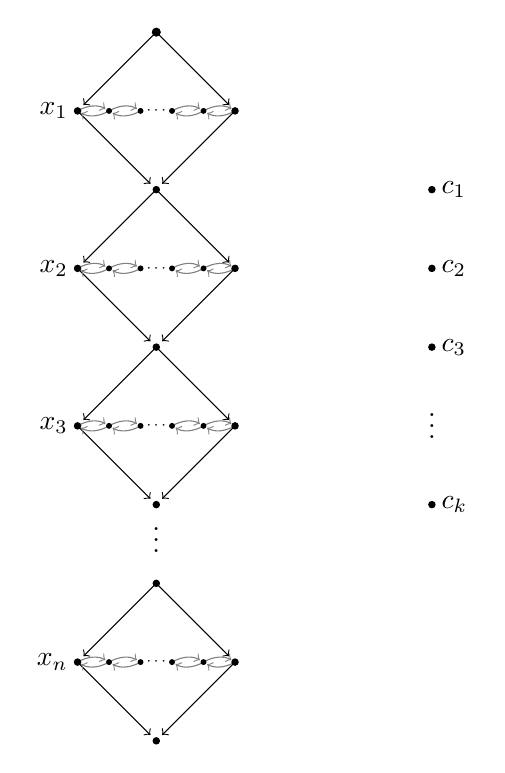
\begin{tikzpicture}
			\draw[fill] (0, 1) circle[radius=0.05];
			\foreach \i in {0, 2, 4, 7}{
				\begin{scope}[shift={(0, -\i)}, ->]
					\begin{scope}[shorten >=3pt]
						\draw (0, 1) -- (1, 0);
						\draw (0, 1) -- (-1, 0);
						\draw (1, 0) -- (0, -1);
						\draw (-1, 0) -- (0, -1);
					\end{scope}
					
					\begin{scope}[shorten >=1.5pt, gray]
						\draw (-1, 0) to[bend left] (-0.6, 0);
						\draw (-0.6, 0) to[bend left] (-0.2, 0);
						\draw (0.6, 0) to[bend left] (1, 0);
						\draw (0.2, 0) to[bend left] (0.6, 0);
						\draw (1, 0) to[bend left] (0.6, 0);
						\draw (0.6, 0) to[bend left] (0.2, 0);
						\draw (-0.6, 0) to[bend left] (-1, 0);
						\draw (-0.2, 0) to[bend left] (-0.6, 0);
					\end{scope}

					\draw[fill] (1, 0) circle[radius=0.04];
					\draw[fill] (-1, 0) circle[radius=0.04];
					\draw[fill] (0, -1) circle[radius=0.04];
					\draw[fill] (-0.6, 0) circle[radius=0.03];
					\draw[fill] (-0.2, 0) circle[radius=0.03];
					\draw[fill] (0.2, 0) circle[radius=0.03];
					\draw[fill] (0.6, 0) circle[radius=0.03];

					\node () {\scalebox{0.6}{\(\cdots\)}};
				\end{scope}
			}
			\node at (0, -5.35) {\(\vdots\)};
			\draw[fill] (0, -6) circle[radius=0.04];

			\node[anchor=east] at (-1, 0) {\(x_1\)};
			\node[anchor=east] at (-1, -2) {\(x_2\)};
			\node[anchor=east] at (-1, -4) {\(x_3\)};
			\node[anchor=east] at (-1, -7) {\(x_n\)};

			\draw[fill] (3.5, -1) circle[radius=0.04] node[anchor=west] {\(c_1\)};
			\draw[fill] (3.5, -2) circle[radius=0.04] node[anchor=west] {\(c_2\)};
			\draw[fill] (3.5, -3) circle[radius=0.04] node[anchor=west] {\(c_3\)};
			\node at (3.5, -3.9) {\(\vdots\)};
			\draw[fill] (3.5, -5) circle[radius=0.04] node[anchor=west] {\(c_k\)};
		\end{tikzpicture}
	\end{center}
	We have diamond structures corresponding to each variable, and a node corresponding to each clause. We want to encode the fact that \(\phi\) is either satisfiable or not satisfiable with a Hamiltonian path. Overall, we will start at \(x_1\), and work our way down to \(x_n\). Let's look at one of the diamond structures more closely.
	\begin{center}
		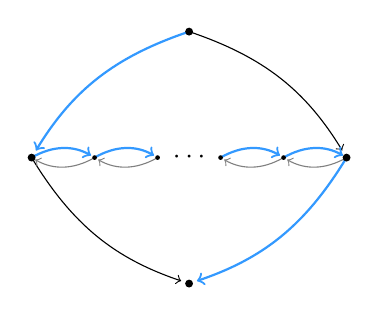
\begin{tikzpicture}[scale=2, ->]
			\definecolor{pathcolor}{rgb}{0.2, 0.6, 1}
			\begin{scope}[shorten >=3pt]
				\draw (0, 0.8) to[bend left=20] (1, 0);
				\draw[pathcolor, line width=0.8pt] (0, 0.8) to[bend right=20] (-1, 0);
				\draw[pathcolor, line width=0.8pt] (1, 0) to[bend left=20] (0, -0.8);
				\draw (-1, 0) to[bend right=20] (0, -0.8);
			\end{scope}
			\begin{scope}[shorten >=1.5pt, gray]
				\draw[pathcolor, line width=0.8pt] (-1, 0) to[bend left] (-0.6, 0);
				\draw[pathcolor, line width=0.8pt] (-0.6, 0) to[bend left] (-0.2, 0);
				\draw[pathcolor, line width=0.8pt] (0.2, 0) to[bend left] (0.6, 0);
				\draw[pathcolor, line width=0.8pt] (0.6, 0) to[bend left] (1, 0);
				\draw (1, 0) to[bend left] (0.6, 0);
				\draw (0.6, 0) to[bend left] (0.2, 0);
				\draw (-0.2, 0) to[bend left] (-0.6, 0);
				\draw (-0.6, 0) to[bend left] (-1, 0);
			\end{scope}
			\fill (0, 0.8) circle[radius=0.025];
			\fill (0, -0.8) circle[radius=0.025];
			\fill (1, 0) circle[radius=0.025];
			\fill (-1, 0) circle[radius=0.025];
			\fill (-0.6, 0) circle[radius=0.015];
			\fill (-0.2, 0) circle[radius=0.015];
			\fill (0.2, 0) circle[radius=0.015];
			\fill (0.6, 0) circle[radius=0.015];

			\node () {\(\cdots\)};
		\end{tikzpicture}
		\qquad
		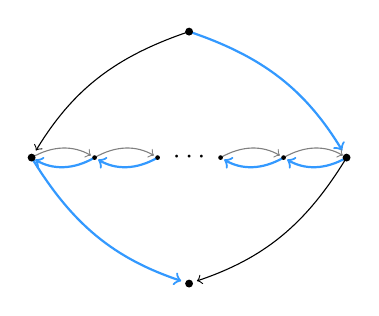
\begin{tikzpicture}[scale=2, ->]
			\definecolor{pathcolor}{rgb}{0.2, 0.6, 1}
			\begin{scope}[shorten >=3pt]
				\draw[pathcolor, line width=0.8pt] (0, 0.8) to[bend left=20] (1, 0);
				\draw (0, 0.8) to[bend right=20] (-1, 0);
				\draw (1, 0) to[bend left=20] (0, -0.8);
				\draw[pathcolor, line width=0.8pt] (-1, 0) to[bend right=20] (0, -0.8);
			\end{scope}
			\begin{scope}[shorten >=1.5pt, gray]
				\draw (-1, 0) to[bend left] (-0.6, 0);
				\draw (-0.6, 0) to[bend left] (-0.2, 0);
				\draw (0.2, 0) to[bend left] (0.6, 0);
				\draw (0.6, 0) to[bend left] (1, 0);
				\draw[pathcolor, line width=0.8pt] (1, 0) to[bend left] (0.6, 0);
				\draw[pathcolor, line width=0.8pt] (0.6, 0) to[bend left] (0.2, 0);
				\draw[pathcolor, line width=0.8pt] (-0.2, 0) to[bend left] (-0.6, 0);
				\draw[pathcolor, line width=0.8pt] (-0.6, 0) to[bend left] (-1, 0);
			\end{scope}
			\fill (0, 0.8) circle[radius=0.025];
			\fill (0, -0.8) circle[radius=0.025];
			\fill (1, 0) circle[radius=0.025];
			\fill (-1, 0) circle[radius=0.025];
			\fill (-0.6, 0) circle[radius=0.015];
			\fill (-0.2, 0) circle[radius=0.015];
			\fill (0.2, 0) circle[radius=0.015];
			\fill (0.6, 0) circle[radius=0.015];

			\node () {\(\cdots\)};
		\end{tikzpicture}
	\end{center}
	There are two ways in which we can go through a diamond structure. In particular, we can go left initially, go right through the internal nodes, and then left to get to the bottom node. Alternatively, we can go right initially and then everything gets flipped. Intuitively, this can correspond to whether the variable is set to true or false.
	
	Now we want to actually encode the information of the formula and clauses being satisfied. In particular, we will visit the node corresponding to the clause if it is satisfied. Then it makes sense that if all the nodes are visited, all of the clauses are satisfied, and furthermore the formula is satisfied.

	In particular, if the clause \(c_i\) contains the literal \(x_j\), then we will connect the structure of \(c_i\) to \(x_j\) as follows:
	\begin{center}
		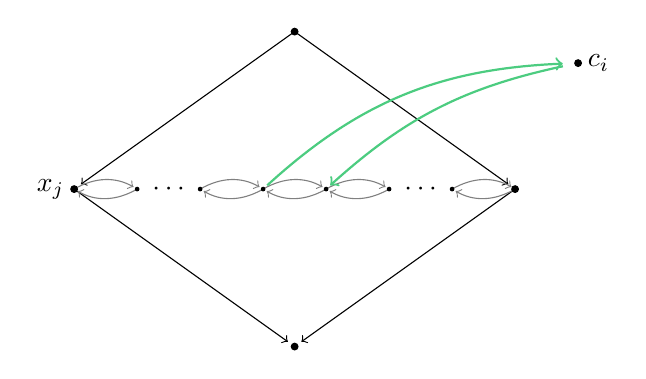
\begin{tikzpicture}[scale=2, ->]
			\definecolor{pathcolor}{rgb}{0.2, 0.6, 1}
			\begin{scope}[shorten >=3pt]
				\draw (0, 1) -- (1.4, 0);
				\draw (0, 1) -- (-1.4, 0);
				\draw (1.4, 0) -- (0, -1);
				\draw (-1.4, 0) -- (0, -1);
			\end{scope}
			\begin{scope}[shorten >=1.5pt, gray]
				\draw (-1.4, 0) to[bend left] (-1.0, 0);
				\draw (-1, 0) to[bend left] (-1.4, 0);

				\draw (-0.6, 0) to[bend left] (-0.2, 0);
				\draw (-0.2, 0) to[bend left] (-0.6, 0);

				\draw (-0.2, 0) to[bend left] (0.2, 0);
				\draw (0.2, 0) to[bend left] (-0.2, 0);

				\draw (0.6, 0) to[bend left] (0.2, 0);
				\draw (0.2, 0) to[bend left] (0.6, 0);

				\draw (1.0, 0) to[bend left] (1.4, 0);
				\draw (1.4, 0) to[bend left] (1, 0);
			\end{scope}
			\fill (0, 1) circle[radius=0.025];
			\fill (0, -1) circle[radius=0.025];
			\fill (1.4, 0) circle[radius=0.025];
			\fill (-1.4, 0) circle[radius=0.025];

			\fill (-1, 0) circle[radius=0.015];
			\fill (-0.6, 0) circle[radius=0.015];
			\fill (-0.2, 0) circle[radius=0.015];
			\fill (0.2, 0) circle[radius=0.015];
			\fill (0.6, 0) circle[radius=0.015];
			\fill (1, 0) circle[radius=0.015];

			\node at (0.8, 0) {\(\cdots\)};
			\node at (-0.8, 0) {\(\cdots\)};

			\node (ci) at (1.8, 0.8) {};
			\fill (ci) circle[radius=0.025];
			\node[anchor=west] at (ci) {\(c_i\)};
			\node[anchor=east] at (-1.4, 0) {\(x_j\)};

			\definecolor{pathcolor}{rgb}{0.3, 0.8, 0.5}
			\begin{scope}[shorten >=2pt, shorten <=2pt, pathcolor, line width=0.8pt]
				\draw (-0.2, 0) to[bend left=20] (ci);
				\draw (ci) to[bend right=15] (0.2, 0);
			\end{scope}
		\end{tikzpicture}
	\end{center}
	Similarly, if the clause \(c_i\) contains the literal \(\neg x_j\), then we connect the structures like so:
	\begin{center}
		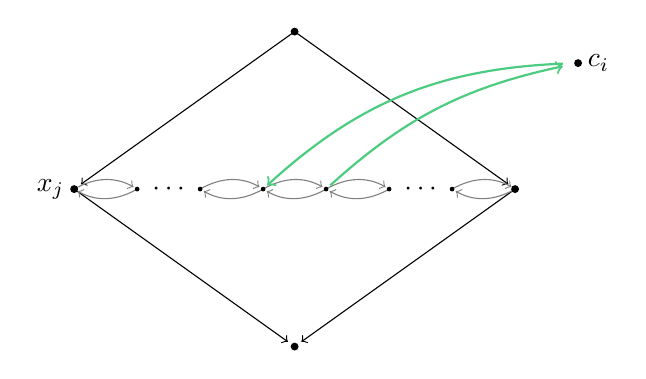
\begin{tikzpicture}[scale=2, ->]
			\definecolor{pathcolor}{rgb}{0.2, 0.6, 1}
			\begin{scope}[shorten >=3pt]
				\draw (0, 1) -- (1.4, 0);
				\draw (0, 1) -- (-1.4, 0);
				\draw (1.4, 0) -- (0, -1);
				\draw (-1.4, 0) -- (0, -1);
			\end{scope}
			\begin{scope}[shorten >=1.5pt, gray]
				\draw (-1.4, 0) to[bend left] (-1.0, 0);
				\draw (-1, 0) to[bend left] (-1.4, 0);

				\draw (-0.6, 0) to[bend left] (-0.2, 0);
				\draw (-0.2, 0) to[bend left] (-0.6, 0);

				\draw (-0.2, 0) to[bend left] (0.2, 0);
				\draw (0.2, 0) to[bend left] (-0.2, 0);

				\draw (0.6, 0) to[bend left] (0.2, 0);
				\draw (0.2, 0) to[bend left] (0.6, 0);

				\draw (1.0, 0) to[bend left] (1.4, 0);
				\draw (1.4, 0) to[bend left] (1, 0);
			\end{scope}
			\fill (0, 1) circle[radius=0.025];
			\fill (0, -1) circle[radius=0.025];
			\fill (1.4, 0) circle[radius=0.025];
			\fill (-1.4, 0) circle[radius=0.025];

			\fill (-1, 0) circle[radius=0.015];
			\fill (-0.6, 0) circle[radius=0.015];
			\fill (-0.2, 0) circle[radius=0.015];
			\fill (0.2, 0) circle[radius=0.015];
			\fill (0.6, 0) circle[radius=0.015];
			\fill (1, 0) circle[radius=0.015];

			\node at (0.8, 0) {\(\cdots\)};
			\node at (-0.8, 0) {\(\cdots\)};

			\node (ci) at (1.8, 0.8) {};
			\fill (ci) circle[radius=0.025];
			\node[anchor=west] at (ci) {\(c_i\)};
			\node[anchor=east] at (-1.4, 0) {\(x_j\)};

			\definecolor{pathcolor}{rgb}{0.3, 0.8, 0.5}
			\begin{scope}[shorten >=2pt, shorten <=2pt, pathcolor, line width=0.8pt]
				\draw (0.2, 0) to[bend left=15] (ci);
				\draw (ci) to[bend right=20] (-0.2, 0);
			\end{scope}
		\end{tikzpicture}
	\end{center}

	We have to be a bit careful about which internal nodes we connect the \(c_i\) node to. In particular, if we don't want them to interfere, we can have \(3k + 3\) nodes, where the \(i\)th clause connects to the \(3i\)th node and \((3i + 1)\)th node. This way, there is a buffer node between everything.

	It is clear that if there is a satisfying assignment, then there will exist a Hamiltonian path through this graph, because we will choose which way we go through each diamond structure, and since each clause is satisfied, we we can visit each clause at some point while zig-zagging through the diamond structures.

	Similarly, if there exists a Hamiltonian path, then we can find the assignment of variables by looking at which direction the path takes through the diamond structures.
\end{proof}



\end{document}

